%%%%%%%%%%%%%%%%%%%%%%%%%%%%%%%%%%%%%%%%%%%%%%
% Lab report template.
%%%%%%%%%%%%%%%%%%%%%%%%%%%%%%%%%%%%%%%%%%%%%%

\documentclass[aps,letterpaper,10pt]{revtex4}

\usepackage{subfigure}
\usepackage{wrapfig}
\usepackage{graphicx} % For images
\usepackage{float}    % For tables and other floats
\usepackage{verbatim} % For comments and other
\usepackage{amsmath}  % For math
\usepackage{amssymb}  % For more math
\usepackage{fullpage} % Set margins and place page numbers at bottom center
\usepackage{listings} % For source code
\usepackage{subfig}   % For subfigures
\usepackage[usenames,dvipsnames]{color} % For colors and names

\definecolor{mygrey}{gray}{.96} % Light Grey
\lstset{ 
    language= Matlab,               % choose the language of the code ("language=Verilog" is %popular as well)
    tabsize=3,    					% sets the size of the tabs in spaces (1 Tab %is replaced with 3 spaces)
	basicstyle=\tiny,               % the size of the fonts that are used for the code
	numbers=left,                   % where to put the line-numbers
	numberstyle=\tiny,              % the size of the fonts that are used for the line-numbers
	stepnumber=2,                   % the step between two line-numbers. If it's 1 each line will %be numbered
	numbersep=5pt,                  % how far the line-numbers are from the code
	backgroundcolor=\color{mygrey}, % choose the background color. You must add %\usepackage{color}
	frame=single,	                % adds a frame around the code
	tabsize=3,	                    % sets default tabsize to 2 spaces
	captionpos=b,                   % sets the caption-position to bottom
	breaklines=true,                % sets automatic line breaking
	breakatwhitespace=false,        % sets if automatic breaks should only happen at whitespace
	%escapeinside={\%*}{*)},        % if you want to add a comment within your code
	commentstyle=\color{BrickRed}   % sets the comment style
}



% TITLE PAGE CONTENT %%%%%%%%%%%%%%%%%%%%%%%%
% Remember to fill this section out for each
% lab write-up.
%%%%%%%%%%%%%%%%%%%%%%%%%%%%%%%%%%%%%%%%%%%%%
\newcommand{\labno}{02}
\newcommand{\labtitle}{Factory Simulation}
\newcommand{\authorname}{Ahmed Kotb (11), Ahmed Mohsen (14), Amr Sharaf (42)}
\newcommand{\professor}{Dr.Sahar Ghanem, Eng.Ahmed Essam}
\newcommand{\classno}{CS433: Performance Evaluation}
% END TITLE PAGE CONTENT %%%%%%%%%%%%%%%%%%%%

% Make units a little nicer looking and faster to type
\newcommand{\Hz}{\textsl{Hz}}
\newcommand{\KHz}{\textsl{KHz}}
\newcommand{\MHz}{\textsl{MHz}}
\newcommand{\GHz}{\textsl{GHz}}
\newcommand{\ns}{\textsl{ns}}
\newcommand{\ms}{\textsl{ms}}
\newcommand{\s}{\textsl{s}}

\begin{document}  % START THE DOCUMENT!


% TITLE PAGE %%%%%%%%%%%%%%%%%%%%%%%%%%%%%%%%%%%%%%
% If you'd like to change the content of this,
% do it in the "TITLE PAGE CONTENT" directly above
% this message
%%%%%%%%%%%%%%%%%%%%%%%%%%%%%%%%%%%%%%%%%%%%%%%%%%%
\begin{titlepage}
\begin{center}

\includegraphics[width=2cm]{Logo_Alexandria_University.jpg}\\
{\LARGE \textsc{Assignment No. \labno:} \\ \vspace{4pt}}
{\Large \textsc{\labtitle} \\ \vspace{4pt}} 
\rule[13pt]{\textwidth}{1pt} \\ \vspace{150pt}
{\large By: \authorname \\ \vspace{10pt}
Instructors: \professor \\ \vspace{10pt}
\classno \\ \vspace{10pt}
\today}
\end{center}
\end{titlepage}
% END TITLE PAGE %%%%%%%%%%%%%%%%%%%%%%%%%%%%%%%%%%
%\tableofcontents
%\newpage


%%%%%%%%%%%%%%%%%%%%%%%%%%%%%%
%%%%%%%%%%%%%%%%%%%%%%%%%%%%%%
\section{Introduction}
%No Text Here
%%%%%%%%%%%%%%%%%%%%%%%%%%%%%%%
\subsection{Purpose}
In this assignment, basic simulation techniques has been used to analyze and evaluate the performance of a factory. The factory consists of a machining center and inspection station in series. Unfinished parts arrive at the factory with exponential interarrival times with a mean of 1 minute. Processing times at the machining center are uniform on the interval [0.65, 0.70] minute, and subsequent inspection times are uniformly distributed as [0.75, 0.80] minute. Ten percent of the parts are bad and are sent back to the machine for rework (i.e. 90% of the
inspected parts are good and are sent to shipping).

The machining center is subject to randomly occurring breakdowns. In particular, a new (or a
freshly-repaired) machine will break down after an exponential amount of time with a mean of 6 hours. Repair times are uniform on the interval [8, 12] minutes. If a part is being processed when the machine breaks down, then the machine continues where it left off upon the completion of repair. The factory is initially empty and idle, and is working continuously without any breaks periods.
%%%%%%%%%%%%%%%%%%%%%%%%%%%%%%
\subsection{Tools/Languages Used}
    \begin{itemize}
        \item{JavaSE for simulation code}
        \item{Matlab for analysis}
    \end{itemize}
%%%%%%%%%%%%%%%%%%%%%%%%%%%%%%

\newpage
\section{Random Number Generation}
\subsection{Primary LCG Used}
    \[x_{n} = 7^5 x_{n-1} mod (2^{31} -1)\]
    This LCG has been used for its long period (2147483647) which is needed to
    generate the seeds for uniform and exponential random generators with
    sufficient non-overlapping periods.
\subsection{Seed Generation}
    Seed Generation is a process that is done once at the beginning of the
    simulation to generate a sufficient number of seeds (currently set to 100
    seeds).
    The LCG described in the previous section (with a seed equals to 1) is used to generate random
    numbers and we only store numbers that are 100,000 apart as seeds (eg.
    $x_{1}$ , $x_{100,001}$ , $x_{200,001}$ , ... ).
    During the simulation the Seed Generator acts as a provider for seeds for
    various uses illustrated in the next 2 sections.
    This technique guarantees that random numbers' generators created with
    different seeds will never overlap (as long as they are used less than
    100,000 times).
\subsection{Uniform Random Generator}
    Uniform Random generation is created by initializing a new instance of the
    Primary LCG described above with a new seed obtained from the seed
    generator.

    To obtain uniform random numbers in a given interval $(a,b)$ the uniform
    random number generator generates a new random number using the LCG and
    divides it by the LCG period to obtain a real number from 0 to 1 ($u$), then
    applies the next formula to get a new number in the desired range.
    \[(b-a)*u + a\]
\subsection{Exponential Random Generator}
    The exponential random number generator is also initialized by creating a
    new instance of the Primary LCG with a new seed obtained from the seed
    generator.

    Exponential Random generator uses the Inverse CDF (Commutative Density
    Function) method to generate random numbers that are exponentially
    distributed.

    Each time a new random number is required the exponential random number
    generator generates a new random real number $u$ from 0 to 1 (as described in
    the previous section) and uses the following inverse CDF equation.
    \[\frac{-1}{\lambda} * ln (u)\]



%%%%%%%%%%%%%%%%%%%%%%%%%%%%%%
%%%%%%%%%%%%%%%%%%%%%%%%%%%%%%
%%%%%%%%%%%%%%%%%%%%%%%%%%%%%%
\newpage
\section{Performance Analysis Procedure}
    \subsection{TCP Connection}
This section will describe the analytical steps done on the experiment data of the TCP connection\\
Definitions:
    \begin{enumerate}
        \item x = sample collected data
        \item n = sample size of collected data
        \item $\bar{x}$ = sample mean 
        \item s = sample deviation 
        \item r = accuracy of number of samples required to follow normal distribution 
        \item CI = confedence IntervaL 
    \end{enumerate}
    \subsubsection{The mean bandwidth over several trials}
            \[
            \bar{x} = \sum_{i=1}^n{\frac{x_{i}}{n}}
            \]
        \subsubsection{The 95\% confidence intervals for the mean bandwidth}
            \[
            n > 30
            \]
            \[
            \bar{x} \sim N(\mu , \frac{s}{\sqrt{n}})
            \]
            \[
            z_{1-\frac{\alpha}{2}} = z_{0.975} = 1.96 \cdots Normal Table
            \]
            \[
            s = \frac{1}{n-1}\sum_{i=1}^n{(x_{i} - \bar{x})^2}
            \]
            \[
            CI = \bar{x} \mp z_{1-\frac{\alpha}{2}}\frac{s}{\sqrt{n}}
            \]
        \subsubsection{the number of samples required to obtain the mean bandwidth with 1\% accuracy}
            \[
            r = 1
            \]
            \[
            z = z_{1-\frac{\alpha}{2}} = 1.96
            \]
            \[
            N_{sample} = \lceil (\frac{100*z*s}{r*\bar{x}})^2 \rceil
            \]
           

\newpage
\section{Experiment Data}
This section will consist of the actual analysis of the collected data.  \vspace{5mm}
    \subsection{TCP Connection}
    This matlab script is used to generate the required data in the analysis of TCP connection    
    	\lstinputlisting{tcp.m}
    	\vspace{3mm}
        \newpage
        \subsubsection{LAN Network}
            \paragraph{Readings}
                \begin{center}
                    \begin{tabular}{ ||l || c | c | c | c | c | c | c | c | c | c | c | c | c | c | c | }
                    \hline
                    Trial number & 1 & 2 & 3 & 4 & 5 & 6 & 7 & 8 & 9 & 10 & 11 & 12 & 13 & 14 & 15 \\ \hline
                    Bandwidth(Mbps) & 81.8 & 82.2 & 78.1 & 74.7 & 75.7 & 75.6 & 77.5 & 75.6 & 74.1 & 75.4 & 76.7 & 76.7 & 74.8 & 74.8 & 77.6\\
                    \hline   
                    \hline
                    Trial number & 16 & 17 & 18 & 19 & 20 & 21 & 22 & 23 & 24 & 25 & 26 & 27 & 28 & 29 & 30 \\ \hline 
                    Bandwidth(Mbps) & 77.2 & 75.0 & 76.0 & 75.8 & 74.0 & 76.6 & 77.2 & 75.5 & 82.0 & 76.9 & 75.2 & 76.5 & 76.5 & 76.3 & 76.0\\     
                    \hline    
                    \hline
                    Trial number & 31 & 32 & 33 & 34 & 35 & 36 & 37 & 38 & 39 & 40 & & & & & \\ \hline
                    Bandwidth(Mbps) & 76.6 & 75.3 & 75.3 & 76.5 & 75.9 & 76.3 & 74.1 & 75.4 & 74.7 & 73.5 & & & & &\\
                    \hline
                    \end{tabular}
                \end{center}
                \vspace{3mm}
            \paragraph{Results}
                \begin{itemize}
                    \item $\bar{x} = 76.3 Mbps$
                    \item $s = 1.94$
                    \item $Confidence$ $interval = (75.7 , 76.9)$
                    \item $N_{normal} = 26$
                \end{itemize}
            \vspace{3mm}           
                         \begin{figure}[htp]
                \begin{center}
                    \subfigure[Qunatiltle quantile plot]{
                    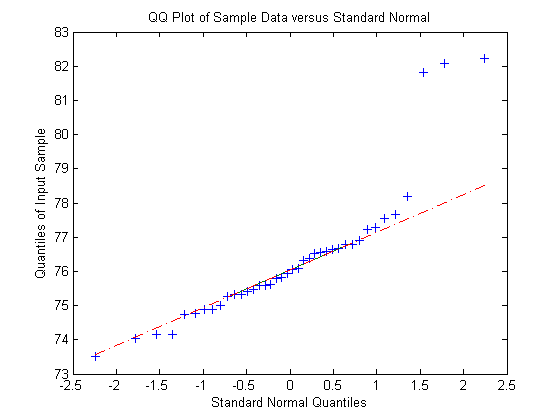
\includegraphics[scale=0.5]{tcp-lan.png}
                    }
                    \subfigure[Histogram plot]{
                    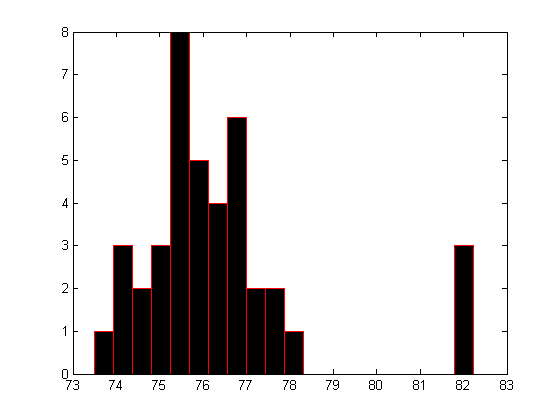
\includegraphics[scale=0.5]{tcp-lan_hist.png}
                    }                        
                \end{center}    
            \end{figure}  
            \paragraph{Observations}
                \begin{itemize}
                        \item Bandwidth is faster than usual DSL 
                        \item according quantile quantile plot the sample data follow noraml distribution
                        \item packet Delay is minimal \textit{i.e.} ad hoc network is used which eliminates the need of a router and therefore the queuing delay and processing delay \\
                        \[
                        d_{nodal} = d_{processing} + d_{queue} + d_{transmission} + d_{propagation}
                        \] 
                        \[
                        d_{processing} = 0 , d_{queue} = 0
                        \] 
                        \item When packet size increase results become more accurate
                        \item the material of the connecting wire affects the limit of the bandwidth
                    \end{itemize}
        \newpage            
        \subsubsection{WLAN Network}
            \paragraph{Readings}
                \begin{center}
                    \begin{tabular}{ ||l || c | c | c | c | c | c | c | c | c | c | c | c | c | c | c | }
                    \hline
                    Trial number & 1 & 2 & 3 & 4 & 5 & 6 & 7 & 8 & 9 & 10 & 11 & 12 & 13 & 14 & 15 \\ \hline
                    Bandwidth(Mbps) & 10.9 & 11.4 & 10.7 & 10.9 & 10.8 & 10.8 & 10.7 & 10.5 & 10.6 & 10.6 & 10.6 & 10.5 & 11.1 & 12.1 & 11.7 \\
                    \hline   
                    \hline
                    Trial number & 16 & 17 & 18 & 19 & 20 & 21 & 22 & 23 & 24 & 25 & 26 & 27 & 28 & 29 & 30 \\ \hline 
                    Bandwidth(Mbps) & 11.7 & 11.5 & 11.7 & 11.5 & 10.7 & 10.4 & 10.6 & 10.5 & 11 & 10.8 & 12.1 & 10.4 & 12 & 10.9 & 10.6 \\ \hline    
                    \hline
                    Trial number & 31 & 32 & 33 & 34 & 35 & 36 & 37 & 38 & 39 & 40 & & & & & \\ \hline
                    Bandwidth(Mbps) & 11 & 11.7 & 12.2 & 11.4 & 12 & 11.7 & 12.3 & 11.9 & 12.1 & 12.2 & & & & &\\
                    \hline
                    \end{tabular}
                \end{center}
                \vspace{3mm}
            \paragraph{Results}
                \begin{itemize}
                    \item $\bar{x} = 11.2 Mbps$
                    \item $s = 0.62$
                    \item $Confidence$ $interval =(11.027 , 11.41) $
                    \item $N_{normal} = 181$
                \end{itemize}
            \vspace{3mm}           
             \begin{figure}[htp]
                \begin{center}
                    \subfigure[Qunatiltle quantile plot]{
                    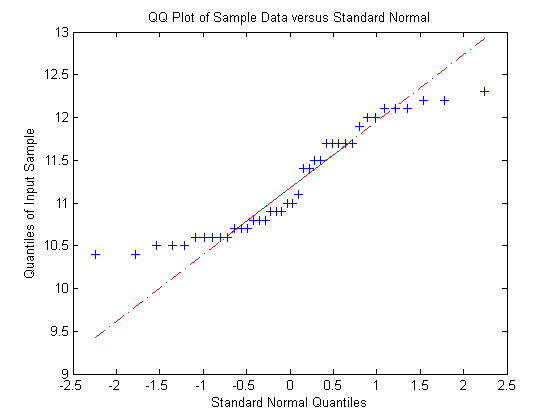
\includegraphics[scale=0.5]{tcp-wifi.png}
                    }
                    \subfigure[Histogram plot]{
                    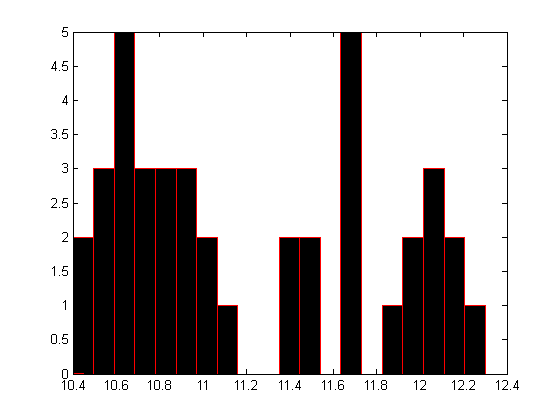
\includegraphics[scale=0.5]{tcp-wifi_hist.png}
                    }                        
                \end{center}    
            \end{figure}   
            \vspace{3mm}
            \paragraph{Observations}
                \begin{itemize}
                        \item Bandwidth is slower than that on lan network 
                        \item According quantile quantile plot the sample data roughly follow noraml distribution
                        \item There exist some noise in the data and this may be due to external factor as the transfer medium
                        \item The results makes more sense when using a wireless ad hoc network rather than that of traditional wifi network
                \end{itemize}
        \newpage        
        \subsubsection{ADSL Network}
            \paragraph{Readings}
                \begin{center}
                    \begin{tabular}{ ||l || c | c | c | c | c | c | c | c | c | c | c | c | c | c | c | }
                    \hline
                    Trial number & 1 & 2 & 3 & 4 & 5 & 6 & 7 & 8 & 9 & 10 & 11 & 12 & 13 & 14 & 15 \\ \hline
                    Bandwidth(Kbps) & 126 & 96.4 & 109 & 114 & 108 & 97.7 & 113 & 113 & 112 & 117 & 112 & 113 & 119 & 85 & 114  \\
                    \hline   
                    \hline
                    Trial number & 16 & 17 & 18 & 19 & 20 & 21 & 22 & 23 & 24 & 25 & 26 & 27 & 28 & 29 & 30 \\ \hline 
                    Bandwidth(Kbps) & 99.7 & 96.2 & 107 & 113 & 117 & 111 & 108 & 103 & 127 & 109 & 119 & 111 & 115 & 103 & 111  \\ \hline    
                    \hline
                    Trial number & 31 & 32 & 33 & 34 & 35 & 36 & 37 & 38 & 39 & 40 & & & & & \\ \hline
                    Bandwidth(Kbps) & 107 & 111 & 106 & 102 & 115 & 108 & 117 & 93.4 & 114 & 103 & & & & &\\
                    \hline
                    \end{tabular}
                \end{center}
                \vspace{3mm}
            \paragraph{Results}
                \begin{itemize}
                    \item $\bar{x} = 109.3 Kpbs$
                    \item $s = 8.43$
                    \item $Confidence$ $interval =(106.7 , 112) $
                    \item $N_{normal} = 229$
                \end{itemize}
            \vspace{3mm}           
             \begin{figure}[htp]
                \begin{center}
                    \subfigure[Qunatiltle quantile plot]{
                    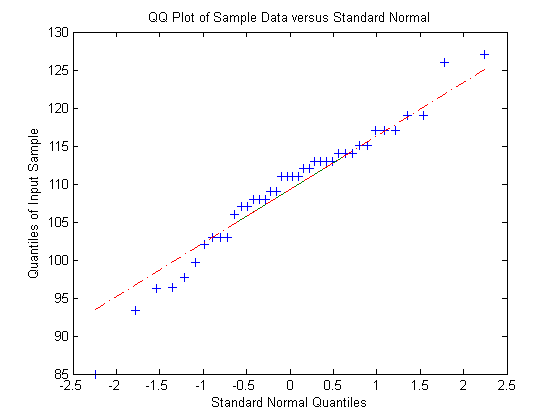
\includegraphics[scale=0.5]{tcp-dsl.png}
                    }
                    \subfigure[Histogram plot]{
                    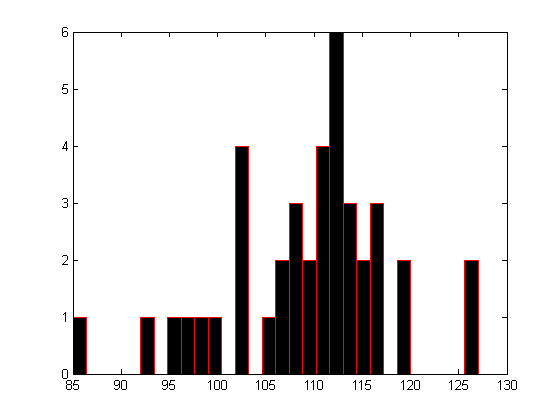
\includegraphics[scale=0.5]{tcp-dsl_hist.png}
                    }                        
                \end{center}    
            \end{figure}   
            \vspace{3mm}
            \paragraph{Observations}
                \begin{itemize}
                        \item Bandwidth is slower than both of lan and wlan nerworks
                        \item According quantile quantile plot the sample data roughly follow noraml distribution
                        \item Readings depends on the router of the server machine and its max bandwidth and whether its overloaded or not
                \end{itemize}
        \newpage
        \subsubsection{Dial up Network}
            \paragraph{Readings}
                \begin{center}
                    \begin{tabular}{ ||l || c | c | c | c | c | c | c | c | c | c | c | c | c | c | c | }
                    \hline
                    Trial number & 1 & 2 & 3 & 4 & 5 & 6 & 7 & 8 & 9 & 10 & 11 & 12 & 13 & 14 & 15 \\ \hline
                    Bandwidth(Kbps) & 87.9 & 87.0 & 99.5 & 106.0 & 93.2 & 64.8 & 101.0 & 106.0 & 101.0 & 100.0 & 106.0 & 94.2 & 93.4 & 100.0 & 114.0  
                    \\ \hline   
                    \hline
                    Trial number & 16 & 17 & 18 & 19 & 20 & 21 & 22 & 23 & 24 & 25 & 26 & 27 & 28 & 29 & 30 \\ \hline 
                    Bandwidth(Kbps) &  89.9 & 69.8 & 100.0 & 105.0 & 104.0 & 105.0 & 109.0 & 89.5 & 94.8 & 102.0 & 105.0 & 64.7 & 6.48 & 9.19 & 98.4  
                    \\ \hline    
                    \hline
                    Trial number & 31 & 32 & 33 & 34 & 35 & 36 & 37 & 38 & 39 & 40 & & & & & \\ \hline
                    Bandwidth(Kbps) & 112.0 & 22.0 & 57.4 & 66.9 & 71.6 & 108.0 & 47.4 & 59.4 & 41.8 & 32.9 & & & & &\\
                    \hline
                    \end{tabular}
                \end{center}
                \vspace{3mm}
            \paragraph{Results}
                \begin{itemize}
                    \item $\bar{x} = 83.1 Kpbs$
                    \item $s = 28.9$
                    \item $Confidence$ $interval =(74.2 , 92.1) $
                    \item $N_{normal} = 4632$
                \end{itemize}
            \vspace{3mm}           
             \begin{figure}[htp]
                \begin{center}
                    \subfigure[Qunatiltle quantile plot]{
                    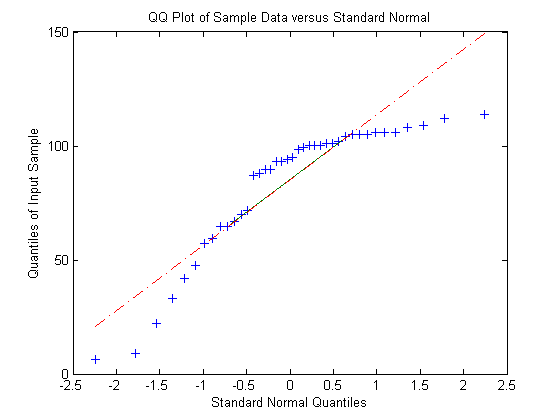
\includegraphics[scale=0.5]{tcp-dailup.png}
                    }
                    \subfigure[Histogram plot]{
                    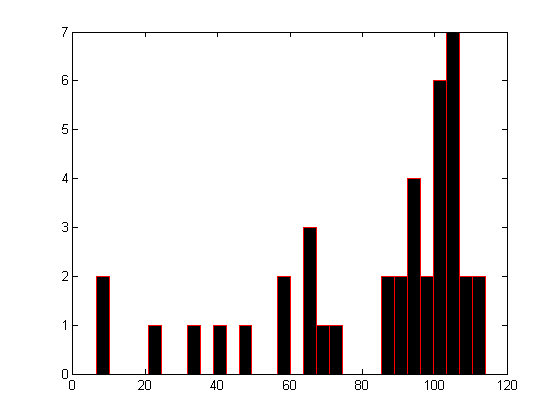
\includegraphics[scale=0.5]{tcp-dailup_hist.png}
                    }                        
                \end{center}    
            \end{figure}   
            \vspace{3mm}
            \paragraph{Observations}
                \begin{itemize}
                        \item Bandwidth is slowest among other networks
                        \item According quantile quantile plot we can assume that the sample data doesn't perfectly follow normal distribution
                 \end{itemize}

\newpage
% UDP SUBSECTION
    \subsection{UDP Connection}
    This batch script is used to collect the required data for UDP analysis using iperf
        \lstinputlisting{run.bat}
    	\vspace{3mm}

        \subsubsection{LAN Network}
            \paragraph{Readings}
                The following table includes the data collected for carrying out the analysis phase for the UDP connection on local area network (LAN). The data rates have been changed from 1 MBytes/sec up to 250 MBytes/sec with a step of 25 MBytes/sec in each iteration. For each data rate, three samples have been collected and the average throughput and loss rate has been recorded.
                \begin{figure}[htp]
                    \begin{center}
                        \subfigure[Readings for UDP Connection in LAN Network]{
                        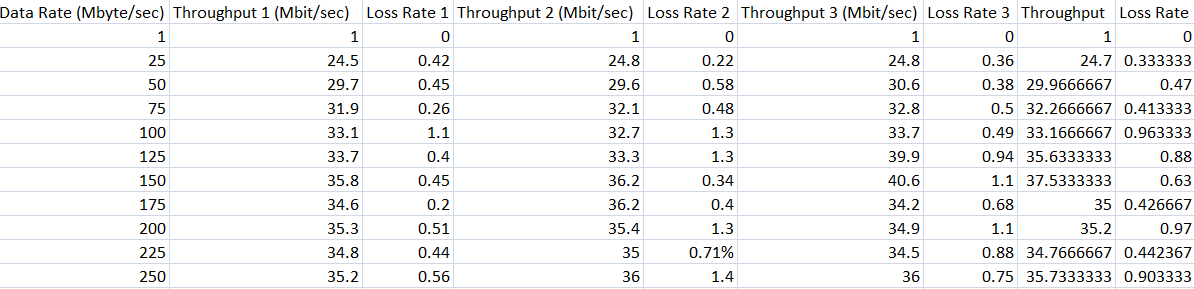
\includegraphics[scale=0.6]{lan-udp-data.png}
                    }             
                    \end{center}    
                \end{figure}            
                \vspace{3mm}
                
            \paragraph{Results}
                The figures below illustrate the realation between the data rate in MBytes/sec and the acheived throughput and loss rate over a local area network (LAN).
                \begin{figure}[htp]
                    \begin{center}
                        \subfigure[Data Rate (MByte/sec)  vs Throughput (Mbps)]{
                            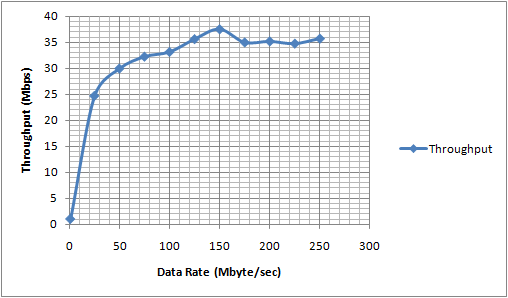
\includegraphics[scale=0.5]{lan-udp-throughput.png}
                        }
                        \subfigure[Loss Rate Percentage]{
                            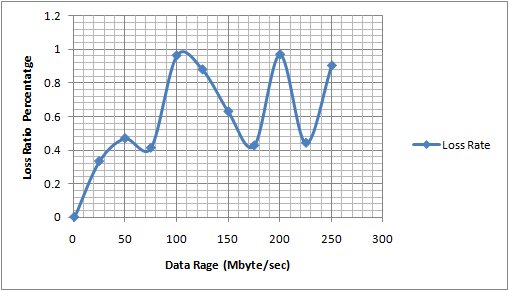
\includegraphics[scale=0.5]{lan-udp-error.png}
                        }                        
                \end{center}    
            \end{figure}
            \paragraph{Observations}
                \begin{itemize}
                        \item Knee Point:
                            \begin{itemize}
                                \item Throughput: 25 Mbps
                                \item Data Rate: 30 MBytes/sec
                            \end{itemize}
                        \item Maximum Throughput: 37 Mbps
                        \item Compared to TCP (76.3 Mbps), it was expected that UDP acheives heigher throughput than TCP. However, due to the default packet size (1470 Bytes / datagram). By increasing the data packet size, the throughput for UDP was improved. Note however that differing nature of UDP and TCP flows means that it their measurements should not be directly compared. Iperf sends UDP datagrams are a constant steady rate, whereas TPC tends to send packet trains. This means that TCP is likely to suffer from congestion effects at a lower data rate than UDP. (\url{http://kb.pert.geant.net/PERTKB/IperfTool})
                        \item The error rate remains within the expected bound (Less than 1 percent). For the error rate below the knee point (30 MBytes/sec), the error increases with the increase in data rate. After the knee point, the error rate behavior tend to be unpredicted but remains heigher than 0.4 percent.
                        \item By changing the direct cable used to connect the two computer devices in the LAN, the UDP and TCP throughput was changed depending on the wire used. Higher quality wires achevied better results reaching up to 90.5 Mbps for TCP and 65 Mbps for UDP.
                \end{itemize}
        \newpage
        \subsubsection{WLAN Network}
            \paragraph{Readings}
                The following table includes the data collected for carrying out the analysis phase for the UDP connection on Wireless local area network (WLAN). The data rates have been changed from 2 MBytes/sec up to 20 MBytes/sec with a step of 2 MBytes/sec in each iteration. For each data rate, three samples have been collected and the average throughput and loss rate has been recorded.
                \begin{figure}[htp]
                        \begin{center}
                            \subfigure[Readings for UDP Connection in WLAN Network]{
                            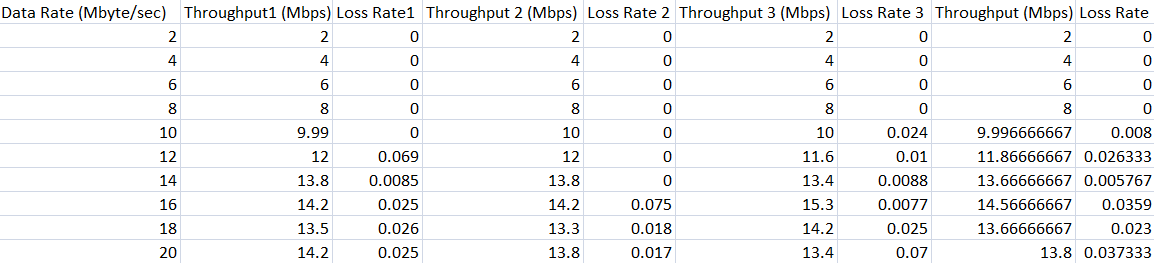
\includegraphics[scale=0.6]{wireless-udp-data.png}
                        }             
                        \end{center}    
                \end{figure}            

                \vspace{3mm}

            \paragraph{Results}
                The figures below illustrate the realation between the data rate in MBytes/sec and the acheived throughput and loss rate over a wireless local area network (WLAN).
                \begin{figure}[htp]
                    \begin{center}
                        \subfigure[Data Rate (MByte/sec)  vs Throughput (Mbps)]{
                            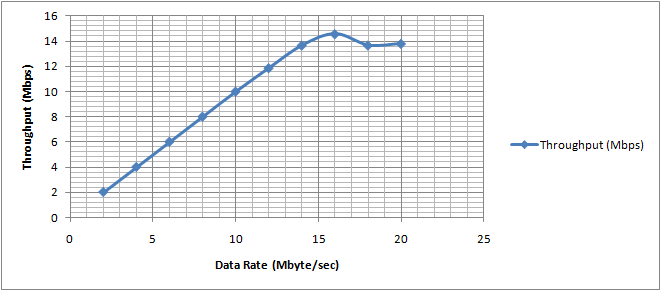
\includegraphics[scale=0.5]{wireless-udp-throughput.png}
                        }
                        \subfigure[Loss Rate Percentage]{
                            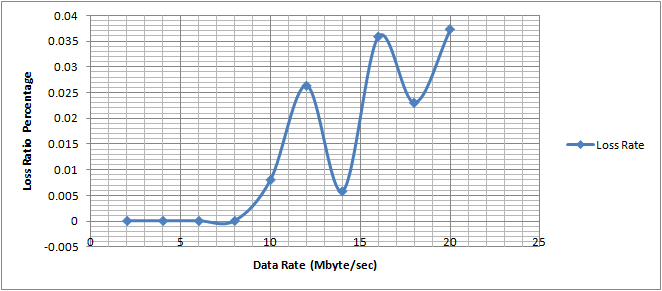
\includegraphics[scale=0.5]{wireless-udp-error.png}
                        }                        
                \end{center}
            \end{figure}
            
            \vspace{3mm}
            
            \paragraph{Observations}
                \begin{itemize}
                        \item Knee Point:
                            \begin{itemize}
                                \item Throughput: 14.5 Mbps
                            \end{itemize}
                        \item Maximum Throughput: 14.5 Mbps
                        \item Compared to TCP (11.2 Mbps), The UDP connection acheived higher throughput compared to TCP (14.5 Mbps)
                        \item The error rate remains within the expected bound (Less than 0.4 percent). It's also clear that the loss rate increases with the increase in the data rate.
                \end{itemize}
        \newpage
        \subsubsection{ADSL Network}
            \paragraph{Readings}
                The following table includes the data collected for carrying out the analysis phase for the UDP connection using ADSL connection. The data rates have been changed from 25 KBytes/sec up to 300 KBytes/sec with a step of 25 KBytes/sec in each iteration. For each data rate, three samples have been collected and the average throughput and loss rate has been recorded.
                \begin{figure}[htp]
                        \begin{center}
                            \subfigure[Readings for UDP Connection in DSL Network]{
                            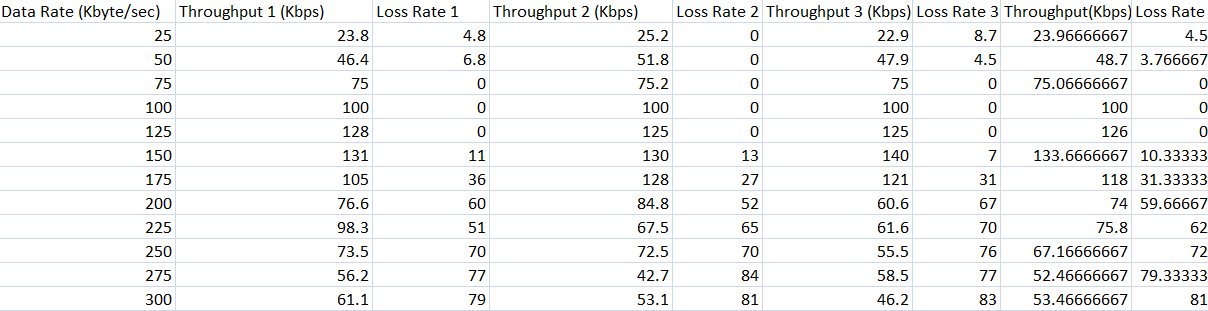
\includegraphics[scale=0.6]{dsl-udp-data.png}
                        }             
                        \end{center}    
                \end{figure}            

            \vspace{3mm}
            
            \paragraph{Results}
                The figures below illustrate the realation between the data rate in MBytes/sec and the acheived throughput and loss rate over a wireless local area network (WLAN).
                \begin{figure}[htp]
                    \begin{center}
                        \subfigure[Data Rate (KByte/sec)  vs Throughput (Kbps)]{
                            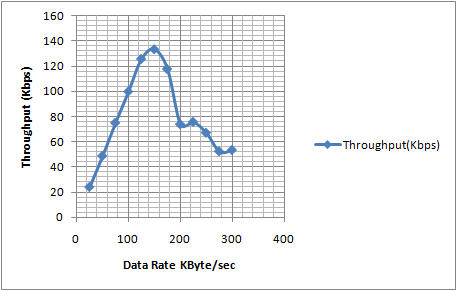
\includegraphics[scale=0.5]{dsl-udp-throughput.png}
                        }
                        \subfigure[Loss Rate Percentage]{
                            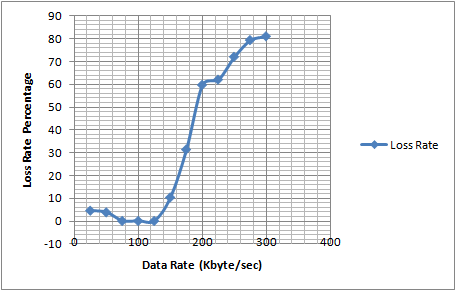
\includegraphics[scale=0.5]{dsl-udp-error.png}
                        }                        
                \end{center}
            \end{figure}
            
            \vspace{3mm}
            
            \paragraph{Observations}
                \begin{itemize}
                        \item Knee Point:
                            \begin{itemize}
                                \item Throughput: 135 Kbps
                            \end{itemize}
                        \item Maximum Throughput: 135 Kbps
                        \item Compared to TCP (109.3 Kbps), The UDP connection acheived higher throughput compared to TCP (135 Kbps)
                        \item It's clear that the loss rate increases with the increase in the data rate. The error reaches 80 Percent for high data transmission rates (300 KBytes/sec)
                \end{itemize}
                
\newpage                
    \section{Conclusion}
        \subsection{TCP}    
            \begin{figure}[htp]
                    \begin{center}
                        \subfigure[Probability plot]{
                        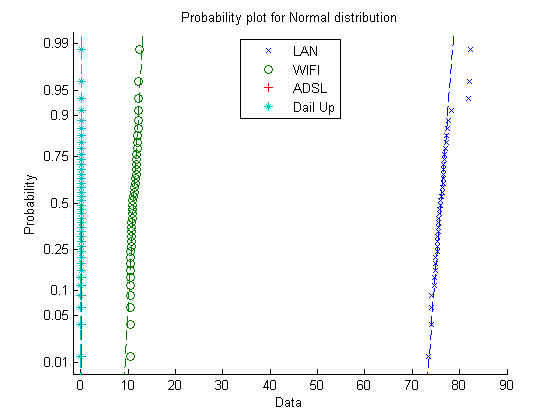
\includegraphics[scale=01]{tcp-all.png}
                        }                        
                    \end{center}    
                \end{figure}   
            \vspace{3mm}
            \begin{center}
                \begin{itemize}
                    \item Performance of wired network is better than that of wireless network
                    \item \[ Bandwidth_{LAN} > Bandwidth_{WLAN} > Bandwidth_{ADSL} > Bandwidth_{Dail up}\]
                    \item The distribution of the Dail up sample data follows the same ditribution as that of ADSL sample data which is not expected but the reason may be that during taking the readings of ADSL experiment the network was congested which cause this low results
                \end{itemize}
            \end{center}

\newpage

        \subsection{UDP}    
            \begin{figure}[htp]
                    \begin{center}
                        \subfigure[Comparison between UDP and TCP]{
                        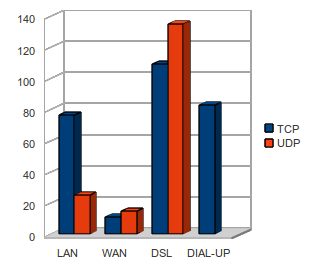
\includegraphics[width=5cm]{comparison.png}
                        }                        
                    \end{center}    
                \end{figure}   
            \begin{center}
                \begin{itemize}
                    \item Performance of UDP connection is better than TCP connection. Although the data collected for the LAN network showed that TCP is faster than UDP, this is not the expected case. This could be due to the packet size assigned for the datagrams and several other different factors.
                    \item \[ Bandwidth_{LAN} > Bandwidth_{WLAN} > Bandwidth_{ADSL} > Bandwidth_{Dail up}\]
                    \item The packet loss ratio increases when the data rate increases.
		  \item It was quite difficult to measure the performance of UDP network over dial-up connection. This is due to the high loss ratio and failure to receive the final server report for the received datagram and loss rate.
                \end{itemize}
            \end{center}
                
                
% IF YOU'D RATHER TYPE THE CODE, OR HAVE A SMALLER BLOCK OF CODE, USE THIS:
%\begin{lstlisting}
%if(something)
%	do this
%else
%	do this
%\end{lstlisting}

%% THIS IS FROM A DIFFERENT CLASS, BUT DEMONSTRATES MATH MODE WELL
%%%%%%%%%%%%%%%%%%%%%%%%%%%%%%
\end{document}
